\chapter{Deuteronomy 3}

\begin{figure}
  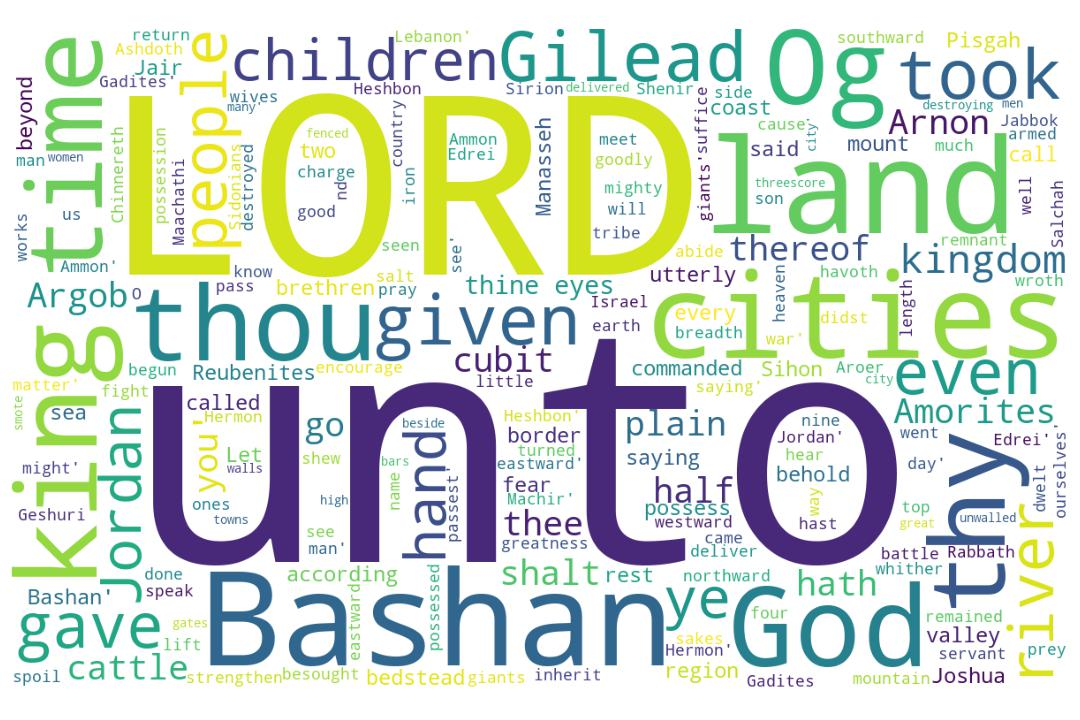
\includegraphics[width=\linewidth]{05OT-Deuteronomy/Deuteronomy3-WordCloud.jpg}
  \caption{Deuteronomy 3 Word Cloud}
  \label{fig:Deuteronomy 3 word Cloud}
\end{figure}


\marginpar{\scriptsize \centering \fcolorbox{bone}{lime}{\textbf{THE END OF THE  BEGINNING}}\\ (Deuteronomy 3:1-29) \begin{compactenum}[I.][8]
    \item   The \textbf{Last} of the Giants \index[scripture]{Deuteronomy!Deu 03:11} (Deu 3:11)
    \item   The \textbf{Lands} for Rueben, Gad, and Manasseh \index[scripture]{Deuteronomy!Deu 03:12--13} (Deu 3:12--13)
        \item   \textbf{Little}  Ones Protected \index[scripture]{Deuteronomy!Deu 03:19} (Deu 3:19)
        \item   \textbf{Lessons}  \index[scripture]{Deuteronomy!Deu 03:21--22} (Deu 3:21--22)
       \item   A \textbf{Lull}  for Moses \index[scripture]{Deuteronomy!Deu 03:26} (Deu 3:26)
\end{compactenum}}

\footnote{\textcolor[cmyk]{0.99998,1,0,0}{\hyperlink{TOC}{Return to end of Table of Contents.}}}\footnote{\href{https://audiobible.com/bible/deuteronomy_3.html}{\textcolor[cmyk]{0.99998,1,0,0}{Deuteronomy 3 Audio}}}\textcolor[cmyk]{0.99998,1,0,0}{Then we turned, and went up the way to Bashan: and Og the king of Bashan came out against us, he and all his people, to battle at Edrei.}
[2] \textcolor[cmyk]{0.99998,1,0,0}{And the LORD said unto me, Fear him not: for I will deliver him, and all his people, and his land, into thy hand; and thou shalt do unto him as thou didst unto Sihon king of the Amorites, which dwelt at Heshbon.}
[3] \textcolor[cmyk]{0.99998,1,0,0}{So the LORD our God delivered into our hands Og also, the king of Bashan, and all his people: and we smote him until none was left to him remaining.}
[4] \textcolor[cmyk]{0.99998,1,0,0}{And we took all his cities at that time, there was not a city which we took not from them, threescore cities, all the region of Argob, the kingdom of Og in Bashan.}
[5] \textcolor[cmyk]{0.99998,1,0,0}{All these cities \emph{were} fenced with high walls, gates, and bars; beside unwalled towns a great many.}
[6] \textcolor[cmyk]{0.99998,1,0,0}{And we utterly destroyed them, as we did unto Sihon king of Heshbon, utterly destroying the men, women, and children, of every city.}
[7] \textcolor[cmyk]{0.99998,1,0,0}{But all the cattle, and the spoil of the cities, we took for a prey to ourselves.}
[8] \textcolor[cmyk]{0.99998,1,0,0}{And we took at that time out of the hand of the two kings of the Amorites the land that \emph{was} on this side Jordan, from the river of Arnon unto mount Hermon;}
[9] \textcolor[cmyk]{0.99998,1,0,0}{\emph{(Which} Hermon the Sidonians call Sirion; and the Amorites call it Shenir;)}
[10] \textcolor[cmyk]{0.99998,1,0,0}{All the cities of the plain, and all Gilead, and all Bashan, unto Salchah and Edrei, cities of the kingdom of Og in Bashan.}
[11] \textcolor[cmyk]{0.99998,1,0,0}{For \fcolorbox{bone}{lime}{only Og} king of Bashan remained of the remnant of giants; behold, his bedstead \emph{was} a bedstead of iron; \emph{is} it not in Rabbath of the children of Ammon? nine cubits \emph{was} the length thereof, and four cubits the breadth of it, after the cubit of a man.}\footnote{The verse states that Og was the last of the remnant of the giants. Apparently another wave of giants arrives later, of which Goliath and his ``brothers'' are.}
[12] \textcolor[cmyk]{0.99998,1,0,0}{And this land, \emph{which} we possessed at that time, from Aroer, which \emph{is} by the river Arnon, and half mount Gilead, and the cities thereof, gave I unto the \fcolorbox{bone}{lime}{Reubenites} and to the \fcolorbox{bone}{lime}{Gadites}.}
[13] \textcolor[cmyk]{0.99998,1,0,0}{And the rest of Gilead, and all Bashan, \emph{being} the kingdom of Og, gave I unto the half tribe of \fcolorbox{bone}{lime}{Manasseh}; all the region of Argob, with all Bashan, which was called the land of giants.}
[14] \textcolor[cmyk]{0.99998,1,0,0}{Jair the son of Manasseh took all the country of Argob unto the coasts of Geshuri and Maachathi; and called them after his own name, Bashan-havoth-jair, unto this day.}
[15] \textcolor[cmyk]{0.99998,1,0,0}{And I gave Gilead unto Machir.}
[16] \textcolor[cmyk]{0.99998,1,0,0}{And unto the Reubenites and unto the Gadites I gave from Gilead even unto the river Arnon half the valley, and the border even unto the river Jabbok, \emph{which} \emph{is} the border of the children of Ammon;}
[17] \textcolor[cmyk]{0.99998,1,0,0}{The plain also, and Jordan, and the coast \emph{thereof}, from Chinnereth even unto the sea of the plain, \emph{even} the salt sea, under Ashdoth-pisgah eastward.}\\
\\\P \textcolor[cmyk]{0.99998,1,0,0}{And I commanded you at that time, saying, The LORD your God hath given you this land to possess it: ye shall pass over armed before your brethren the children of Israel, all \emph{that} \emph{are} meet for the war.}
[19] \textcolor[cmyk]{0.99998,1,0,0}{But your wives, and your \fcolorbox{bone}{lime}{little ones}, and your cattle, \emph{(for} I know that ye have much cattle,) shall abide in your cities which I have given you;}
[20] \textcolor[cmyk]{0.99998,1,0,0}{Until the LORD have given rest unto your brethren, as well as unto you, and \emph{until} they also possess the land which the LORD your God hath given them beyond Jordan: and \emph{then} shall ye return every man unto his possession, which I have given you.}\\
\\
\P \textcolor[cmyk]{0.99998,1,0,0}{And I commanded Joshua at that time, saying, \fcolorbox{bone}{lime}{Thine eyes have seen} all that the LORD your God hath done unto these two kings: so shall the LORD do unto all the kingdoms whither thou passest.}
[22] \textcolor[cmyk]{0.99998,1,0,0}{Ye shall not fear them: for the LORD your God he shall fight for you.}
[23] \textcolor[cmyk]{0.99998,1,0,0}{And I besought the LORD at that time, saying,}
[24] \textcolor[cmyk]{0.99998,1,0,0}{O Lord GOD, thou hast begun to shew thy servant thy greatness, and thy mighty hand: for what God \emph{is} \emph{there} in heaven or in earth, that can do according to thy works, and according to thy might?}
[25] \textcolor[cmyk]{0.99998,1,0,0}{I pray thee, let me go over, and see the good land that \emph{is} beyond Jordan, that goodly mountain, and Lebanon.}
[26] \textcolor[cmyk]{0.99998,1,0,0}{But the LORD was wroth with me for your sakes, and would not hear me: and the LORD said unto me, Let it suffice thee; \fcolorbox{bone}{lime}{speak no more} unto me of this matter.}
[27] \textcolor[cmyk]{0.99998,1,0,0}{Get thee up into the top of Pisgah, and lift up thine eyes westward, and northward, and southward, and eastward, and behold \emph{it} with thine eyes: for thou shalt not go over this Jordan.}
[28] \textcolor[cmyk]{0.99998,1,0,0}{But charge Joshua, and encourage him, and strengthen him: for he shall go over before this people, and he shall cause them to inherit the land which thou shalt see.}
[29] \textcolor[cmyk]{0.99998,1,0,0}{So we abode in the valley over against Beth-peor.}